\section{Svolgimento}

È stato definito quale tool utilizzare per generare la documentazione Angular.

Compodoc fornisce anche il calcolo della copertura della documentazione rispetto al codice nei progetti Angular:

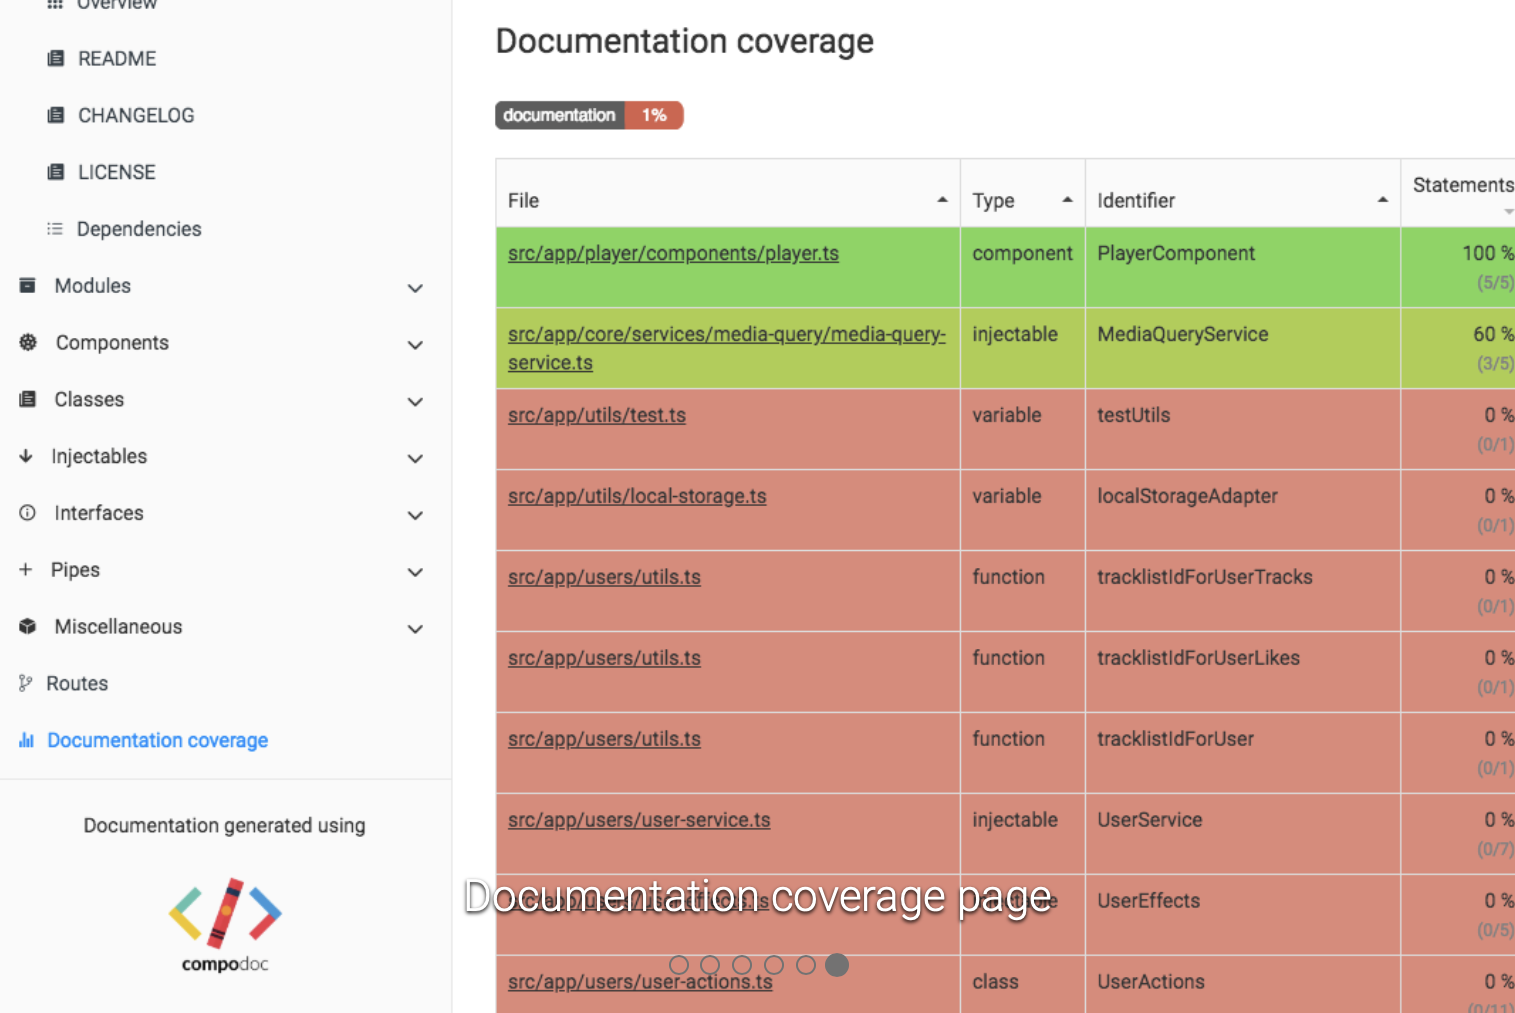
\includegraphics[width = 0.9\linewidth]{img/compodoc.png}

Angular è stato scelto per la realizzazione della WebApp lato front-end, pertanto si è resa necessaria la ricerca di un tool per generare la documentazione relativa a quanto prodotto, necessaria ai fini del progetto.

Abbiamo deciso come gruppo di inserire l'utilizzo di questo strumento nel nostro {\it{Way of Working}} per la stesura della documentazione su Angular.

La documentazione è richiesta come da requisito di qualità RQ\_02 definito nel documento "Analisi dei Requisiti", il quale prevede che il progetto includa un manuale per sviluppatori che fornisca spiegazione dettagliate su come svolgere manutenzione sull'applicativo. Questo requisito, come definito dal capitolato, va rispettato obbligatoriamente.